\subsection{Neural Networks}
\label{sec::321_nn}
Neural networks are inspired by the brain's structure, and as we will see later in this chapter, their building blocks can be thought of as neurons (figure \ref{fig::321_neuron}).
\begin{figure}[h]
	\centering
	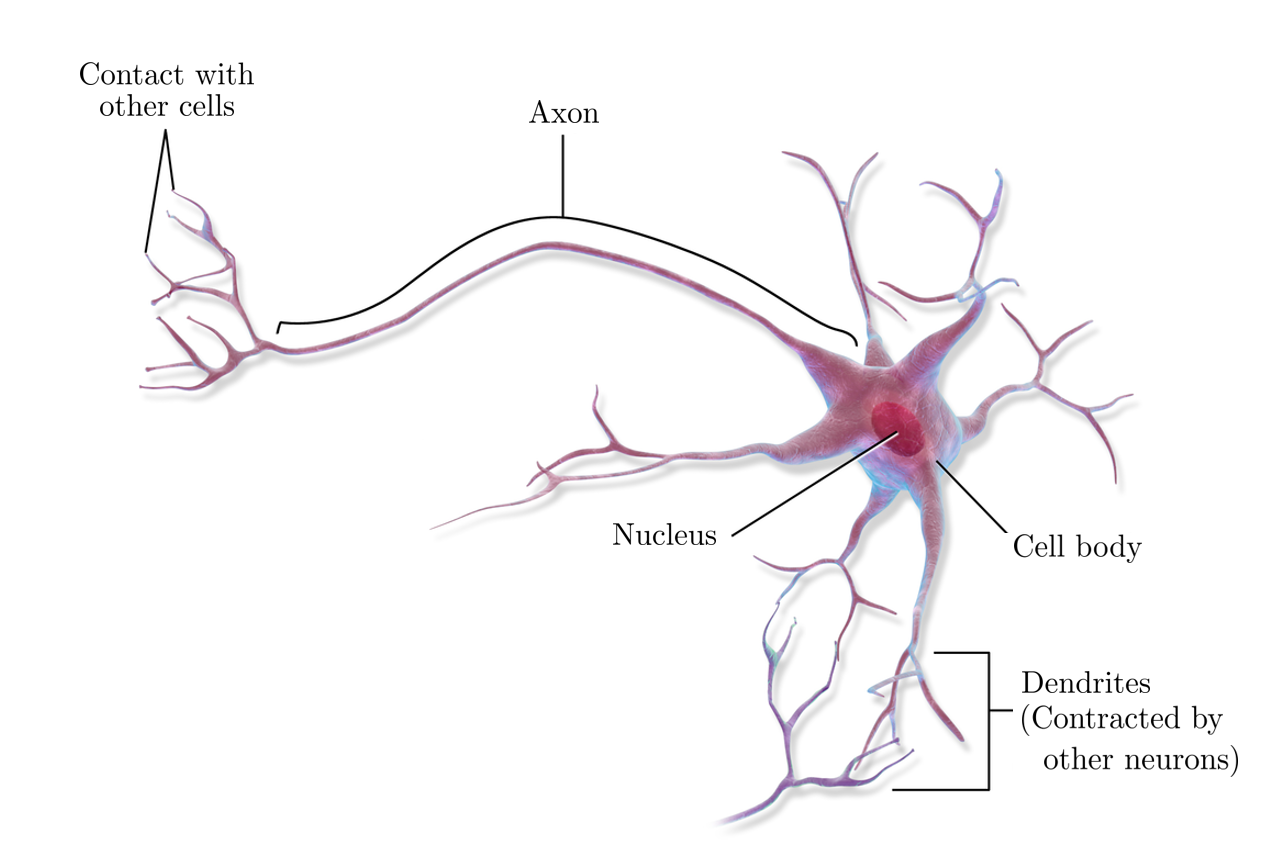
\includegraphics[scale=.35]{chapters/03_background/img/neuron.png}
	\caption{Biological neuron, which connects its cell body to dendrites of surrounding neurons via an axon. \cite{haggstrom2014medical}}
	\label{fig::321_neuron}
\end{figure}
And although neural networks have gained early attention in research, they have only recently become powerful for their implementation on graphic processing units (GPUs) \cite{oh2004gpu}. This was caused by their mathematical description that is linear and can be parallalized very well. Running neural nets on GPUs on the other hand consumes a lot of energy, which stays in contrast to biological neurons, which communicate by brief energy efficient spikes \cite{hodgkin1952quantitative}. And while there are around 100 billion neurons in the human brain, currently huge neural networks have around a factor of 10000 less \cite{goodfellow2016deep}. Not only is the number of neurons in a neural net comparably small, but also is their complexity way below that of a biological neuron. To tackle this discrepancy, and to learn complicated tasks, it is therefore required to introduce activation functions for neural networks, such as the rectifying linear unit \cite{krizhevsky2012imagenet}. This enables neural networks to be used on a variety of problems, but they currently lack in transferring knowledge between different domains, and tend to over-fit certain tasks. There exist methods to deal with this tendency, such as max-pooling \cite{weng1992cresceptron} or dropout \cite{srivastava2014dropout} layers, which efficiently just reduce the number of neurons within a neural net. To build a good understanding of neural networks, we will introduce different architectures in the following that will be used throughout this thesis, and we will start with the simplest in the next paragraph - Fully Connected Neural Network.
\subsubsection{Fully Connected Neural Network}
The biologically inspired perceptron model \cite{viglione19704} lay the foundation for neural networks and it got extended pretty soon to the multi-layer perceptron model
\cite{ivakhnenko1971polynomial}, which is known today as the fully connected neural network. Due to its similarity to the brain's structure, it is often depicted as in figure \ref{fig::321_fully_connected}, where each orange circle represents a neuron that is connected to its surroundings via simple weights $w_{ij}$, as neurons inside the brain are by synapses.
\begin{figure}[h]
	\centering
	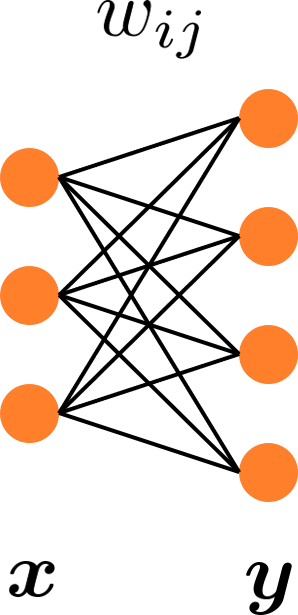
\includegraphics[scale=.28]{chapters/03_background/img/fully_connected.png}
	\caption{Fully connected neural network with three inputs and four outputs. Each orange circle represents what is often referred to as neuron, while the black lines indicate the connections between each neuron.}
	\label{fig::321_fully_connected}
\end{figure}
Mathematically speaking, the feed forward process can be described as a simple matrix multiplication with all weights $\bm{W}$, where the input $\bm{x}$ gets converted to the output $\bm{y}$ via
\begin{align}
	\bm{y} = \bm{W}\bm{x}+\bm{b}
	\label{eq::321_fully_connected}
\end{align}
Therein, the bias $\bm{b}$ can be understood as a shift of isolines that are introduced by hyperplanes. These hyperplanes are learned and expressed by the layer's weights $w_{ij}$ (figure \ref{fig::321_classification}). The output $\bm{y}$, is then further passed through an activation function $f$, and therefore can be compared to the action potential inside a neuron, as it determines the amount by which the next neuron gets excited. This activation function can be anything from a simple step function for classification to a linear function for regression. In practice there are some activation functions that have shown to be of particular use and we will introduce them later in this chapter.
\begin{figure}[h]
	\centering
	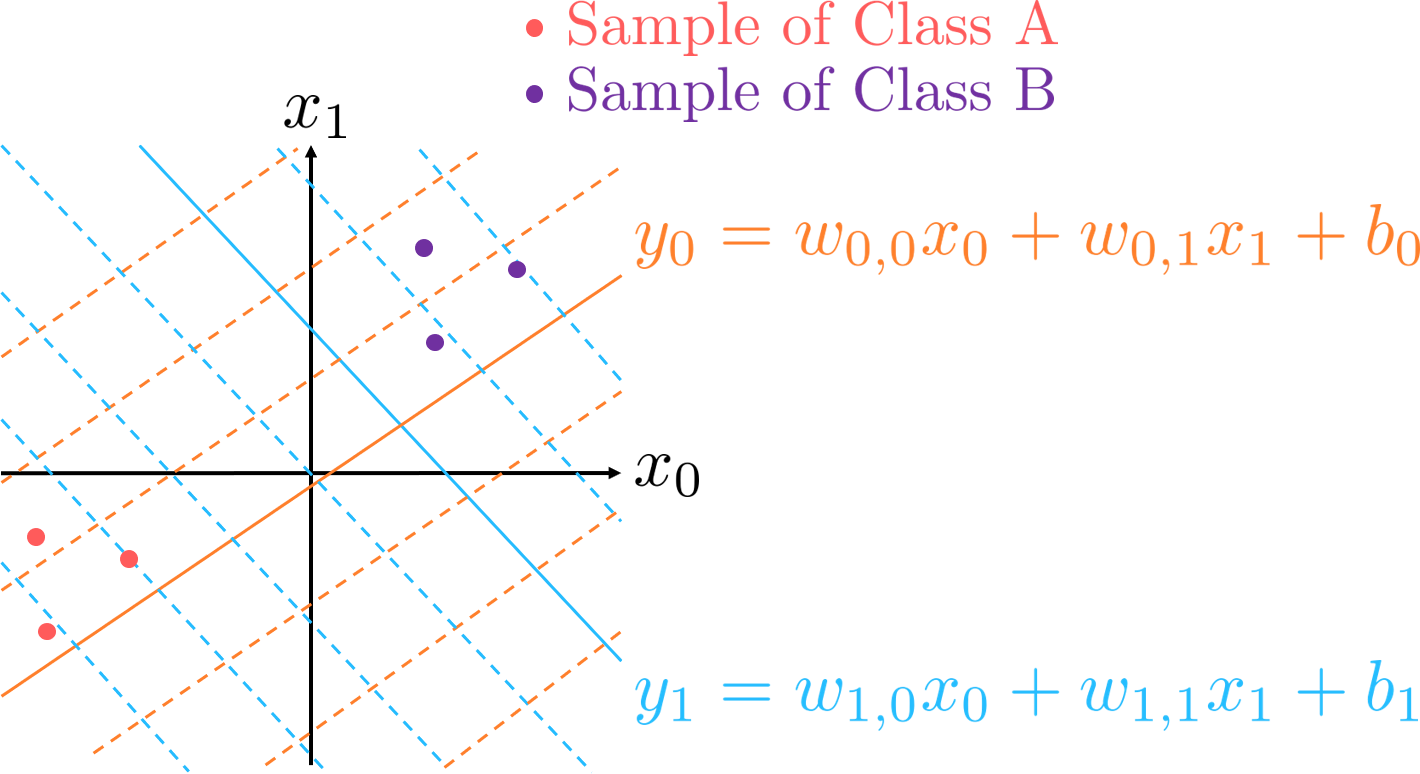
\includegraphics[scale=.28]{chapters/03_background/img/classification.png}
	\caption{Simple interpretation of a fully connected neural network with one layer that takes $\bm{x}=(x_0\,\,x_1)^T$ as input. The dotted lines are isolines to the hyperplane, which showcase the effect of the bias $\bm{b}$.}
	\label{fig::321_classification}
\end{figure}
\subsubsection{Convolutional Neural Network}
The concept of convolutional neural networks was first inspired by biological structures inside the visual cortex of the human brain. It was introduced as neocognitron \cite{fukushima1980neocognitron}, and soon after termed convolutional neural network for its mathematical properties, in that it equals convolutions. Figure \ref{fig::321_convolutional} shows how an input $\bm{x}$ is fed forward through the network architecture across two layers.   
\begin{figure}[h]
	\centering
	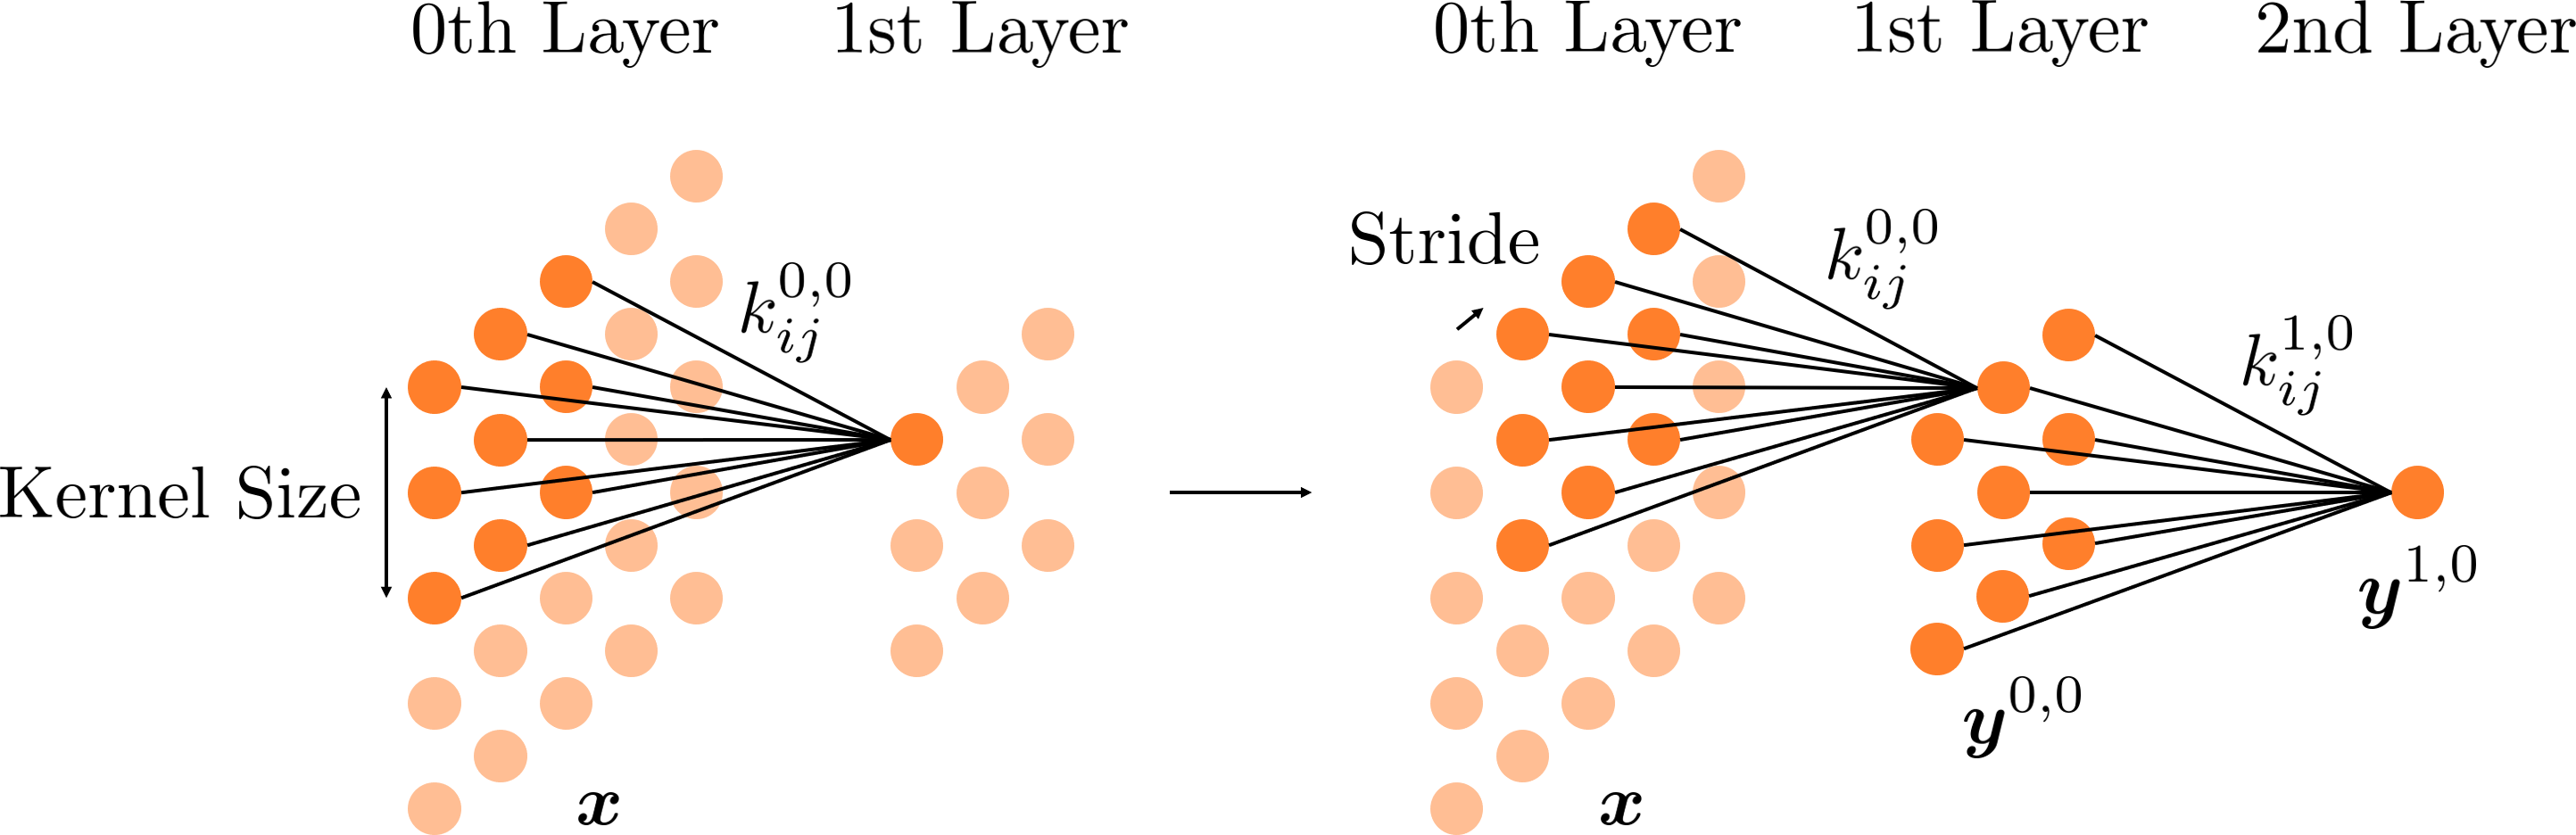
\includegraphics[scale=.28]{chapters/03_background/img/convolutional.png}
	\caption{Convolutional neural network with a total of three layers of which one is the input layer. For visualization, the kernel size is set to be three, and the stride is set to be one.}
	\label{fig::321_convolutional}
\end{figure}
The operation is again visualized by utilizing orange circles, which may be referred to as neurons. These neurons are connected by weights $k^{l,n}_{ij}$, which together constitute the kernel $\bm{k}^{l,n}$ of each convolution. Therein, $l$ stands for the current layer, and $n$ indexes the kernel within a layer, as there may in principle be many different kernels for a single layer. Mathematically speaking, we can formulate the process as follows
\begin{align}
	\bm{y}^{0,0} &= f(\bm{x}*\bm{k}^{0,0}) \\
	\bm{y}^{1,0} &= f(\bm{y}^{0,0}*\bm{k}^{1,0})	
\end{align}
One thing to notice is that the deeper we go, meaning the more layers we have, the more of the initial input contributes to the current activation. This can be seen in figure \ref{fig::321_convolutional}, where each neuron within the first layer only sees a kernel size sized snipped of the original input $\bm{x}$, whereas a neuron within the second layer already sees all of it. This intuitive understanding of convolutional neural networks is backed by visualizations of the highest activity neuron's gradient with respect to the input, where the gradient itself equals the transposed convolution \cite{simonyan2013deep}.  Figure \ref{fig::321_transposed_conv} shows transposed convolutions for a classification network that was trained on ImageNet \cite{deng2009imagenet}. It can be seen that while superficial layers learn to understand edges, deeper layers grab more complex spatial correlations within images, such as car wheels within the third layer.
\begin{figure}[h]
	\centering
	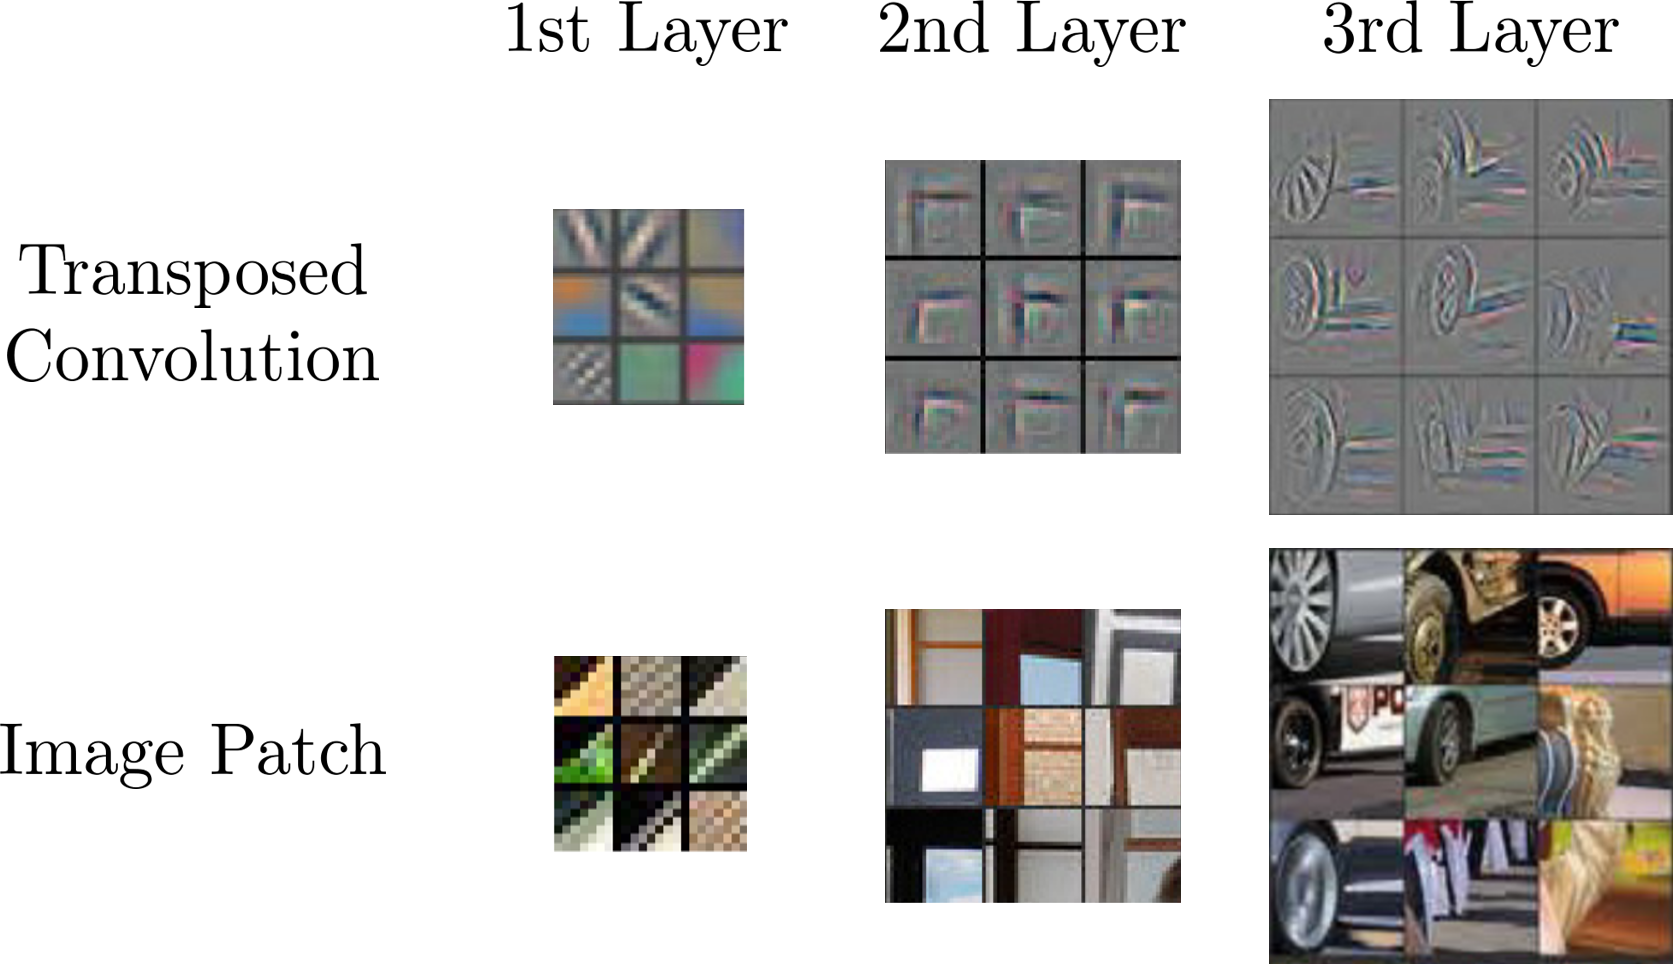
\includegraphics[scale=.28]{chapters/03_background/img/transposed_conv.png}
	\caption{Analysis of neurons with highest activation, corresponding to a subset of ImageNet. For the first layer, the kernel itself is shown, and image patches at the kernel's scale. For the second and third layer, a single neuron with highest activation is upscaled by transposed convolutions to the first layer's feature map. Images taken from \cite{zeiler2014visualizing}.}
	\label{fig::321_transposed_conv}
\end{figure}
Therefore, convolutional neural networks are particularly well suited for understanding spatial correlations, and while recent advancements also propose the promising use of convoltional neural networks for time series analysis \cite{vaswani2017attention}, a simpler approach are long short-term memory units, which will be explained in the next section - Long Short-Term Memory. 
\subsubsection{Long Short-Term Memory}
Long short-term memory units were introduced to overcome the vanishing and exploding gradient problem for recurrent neural networks in time series analysis \cite{hochreiter1997long}. That is the gradient tends to diverge exponentially over the course of the backward pass towards earlier inputs, resulting in intractable updates for the weights of the neural network. This issue got solved by adding a constant recurrent self-connection that allows for constant error propagation through the network, which got further refined by replacing the constant self-connection with a forget gate \cite{gers1999learning}. The inner workings of a long short-term memory unit is shown in figure \ref{fig::321_lstm}. 
\begin{figure}[h]
	\centering
	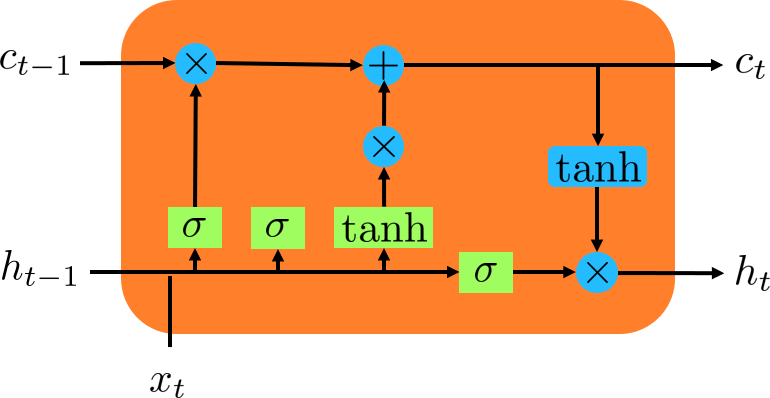
\includegraphics[scale=.28]{chapters/03_background/img/lstm.png}
	\caption{Long short-term memory unit with cell states $\bm{c}_i$, hidden states $\bm{h}_i$, input $\bm{x}_t$, and activation functions $\sigma/\tanh$, as well as addition $+$ and multiplication $\times$ operators.}
	\label{fig::321_lstm}
\end{figure}
The underlying mathematical operations can therein be expressed as follows
\begin{align}
	\bm{i}_t &= \sigma(\bm{W}_{ii}\bm{x}_t+\bm{b}_{ii}+\bm{W}_{hi}\bm{h}_{t-1}+\bm{b}_{hi})\\
	\bm{f}_t &= \sigma(\bm{W}_{if}\bm{x}_t+\bm{b}_{if}+\bm{W}_{hf}\bm{h}_{t-1}+\bm{b}_{hf})\\
	\bm{g}_t &= \tanh(\bm{W}_{ig}\bm{x}_t+\bm{b}_{ig}+\bm{W}_{hg}\bm{h}_{t-1}+\bm{b}_{hg})\\
	\bm{o}_t &= \sigma(\bm{W}_{io}\bm{x}_t+\bm{b}_{io}+\bm{W}_{ho}\bm{h}_{t-1}+\bm{b}_{ho})\\
	\bm{c}_t &= \bm{f}_t\cdot c_{t-1} + \bm{i}_t\cdot\bm{g}_t\\
	\bm{h}_t &= \bm{o}_t \cdot\tanh(\bm{c}_t),
\end{align}
where $\cdot$ is an element-wise multiplication. The sigmoid function $\sigma$, which ranges from 0 to 1, assures that the input gate $\bm{i}_t$, the forget gate $\bm{f}_t$, and the output gate $\bm{o}_t$ let only pass values of interest into, and out of the cell. Multiple long short-term memory units can then be linked for time series analysis as shown in figure \ref{fig::321_lstm_chain}.
\begin{figure}[h]
	\centering
	
\includegraphics[scale=.28]{chapters/03_background/img/lstm_chain.png}
	\caption{Chain of long short-term memory units for temporal understanding of the input sequence $\bm{x}_i$.}
	\label{fig::321_lstm_chain}
\end{figure}
\subsubsection{Backpropagation}
The currently most popular way to train a neural network is backpropagation, which got first introduced in \cite{linnainmaa1970representation}. It has no biological equivalent but poses an effective way to optimize a huge amount of parameters. Newer methods use evolutionary algorithms and treat network parameters as population that develops over time \cite{montana1989training}, but we wont consider them further. The reason for why backpropagation works so well to optimize neural networks, is the simplicity of the mathematical operations that make them up. Not only do the activation functions have an analytical derivative, but further can we just apply the chain rule multiple times on the loss function, so to find the gradient for every network parameter. Suppose we have the loss $L$, then the derivative with respect to the weights $\bm{W}_l$ of layer $l$, is just given as
\begin{align}
	\frac{\partial L}{\partial \bm{W}_l} = \bm{\delta}_l\bm{x}_{l-1}^T,
	\label{eq::321_bp}
\end{align}
where for the last layer $N$, and all previous layers $l$, we have
\begin{align}
	\bm{\delta}_N &= \frac{\partial L}{\partial \bm{x}_N} \cdot f_N'(\bm{W}_N\bm{x}_{N-1}) \\
	\bm{\delta}_l &= \bm{W}^T_{l+1}\bm{\delta}_{l+1} \cdot f_{l}'(\bm{W}_l\bm{x}_{l-1}),
\end{align} % https://sudeepraja.github.io/Neural/
with $f'$ being the derivative of the corresponding activation function. The update for the next time-step $t+1$ is then performed according to an optimizer specific learning rate $\bm{\alpha}_{\bm{W}^t_l}$ as follows
\begin{align}
	\bm{W}_l^{t+1} = \bm{W}_l^t - \bm{\alpha}_{\bm{W}^t_l}\cdot\frac{\partial L}{\partial \bm{W}^l},
\end{align}
where $\cdot$ is an element-wise multiplication.